%!TEX root = ../main.tex
\thispagestyle{ika}

% --- EINLEITUNG ---------------------------------------------------------------
\chapter{Einleitung}

In der Automobilindustrie geht der Trend in den vergangenen Jahren verstärkt  zur Entwicklung und Realisierung von autonomen Fahrfunktionen. Um diese automatisierten Fahrmanöver zu validieren und abzusichern werden Testfahrten mit oft vielen tausend Testkilometern benötigt. Als kostengünstige Alternative zur realen Testfahrt können diese Fahrmanöver auch mithilfe von Simulationen durchgeführt werden. Der Ausgangspunkt bzw. die Grundvoraussetzung für jede Fahrzeugsimulation ist eine vorhandene Streckenbeschreibung auf der die entsprechende Simulation durchgeführt wird. Zum einen können solche Strecken anhand von realen Daten erzeugt werden, was jedoch einen hohen Detaillierungsgrad voraus setzt und aktuell nicht automatisiert realisierbar ist. Eine weitere Möglichkeit zur Erzeugung von Strecken ist ein logisch, variierbarer Ansatz der als Grundlage für diese Seminararbeit herangezogen wird. Hierbei ist nicht das Abbild der Realität das Ziel, sondern Vorschriften und Grenzen einzuhalten und durch einfache und parametrisierte Angaben ein komplexes und vor allem in sich valides Streckennetz generieren zu können.

Die Grundidee dieser Arbeit ist nun die Implementierung eines Tools mithilfe dessen der Benutzer anhand von vereinfachten logischen Streckenbeschreibungen ein konkretes in sich valides Streckennetz erhält. Das Eingabeformat wurde als solches im Rahmen einer Masterarbeit klar definiert und ausgearbeitet \cite{Russ.2019}. Die Hauptaufgabe dieser Seminararbeit besteht nun also in der Validierung und Absicherung des vorhandenen Formates und dem Entwickeln eines Übersetzungstool, dass die konkrete Strecke in einem industriell gängigem Format als Resultat liefert. Besonderer Fokus wird in erster Linie auf innerstädtische Streckenszenarien gelegt, sodass ins besondere Kreuzungen genauer Untersucht werden. 

% --- ALLGEMEINE STRECKENBESCHREIBUNG ------------------------------------------
\chapter{Allgemeine Streckenbeschreibung}

Grundsätzlich lässt sich eine Strecke in verschiedene Ebenen teilen, wie in Abbildung \ref{abb1} sichtbar. Ausgangspunkt ist die Straße als solche mit Fahrbahnen und Fahrbahnmarkierungen. Ein weiterer Bestandteil sind verkehrsführende Elemente wie beispielsweise Beschilderungen, Ampelanlagen oder Bushaltestellen. Ein letzter, für die Streckenbeschreibung notwendiger Aspekt, sind temporäre Veränderungen wie zum Beispiel Baustellen. Alle weiteren Ebenen des gezeigten Modells finden in der Streckenbeschreibung und Generierung keine Anwendung.

\begin{figure}[H]
\flushleft
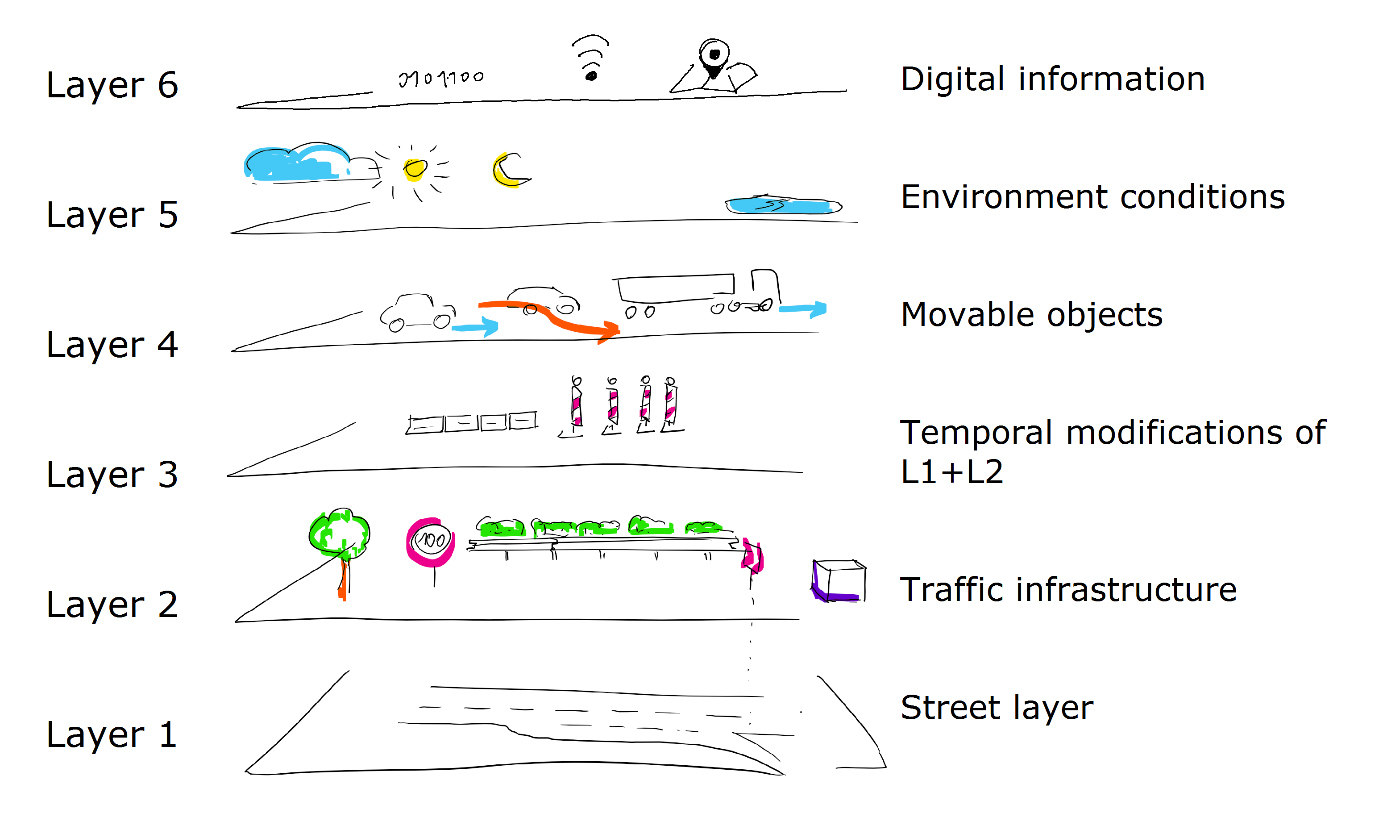
\includegraphics[width=0.95\textwidth]{fig/fig1.png}
\caption{Vereinfachtes Ebenenmodell einer Straße \cite{Eckstein.2018}}
\label{abb1}
\end{figure}

Im Allgemeinen gibt es zwei relevante Koordinatensysteme für Strecken. Neben dem globalen x-y Koordinatensystem existiert das der Referenzlinie mitbewegte s-t Koordinatensystem, wie auch Abbildung \ref{abb2} verdeutlicht. Jede Straße besitzt eine Referenzlinie, deren Beschreibung analytisch durch das Verbinden von Gerade, Kreisbögen und Spiralsegmenten möglich ist. Diese im Straßenbau standardisierte Methode ermöglicht eine kontinuierliche Beschreibung ohne Krümmungsprung. Eine Gerade mit Krümmung Null und ein Kreisbogen mit konstanter Krümmung können durch ein Spiralsegment mit linearem Krümmungsanstieg verbunden werden. Eine beispielhafte Referenzlinie ist hierbei in Abbild \ref{abb2} dargestellt, wobei das unten dargestellte Krümmungsband wie erläutert stetig ist.

\begin{figure}[H]
\flushleft
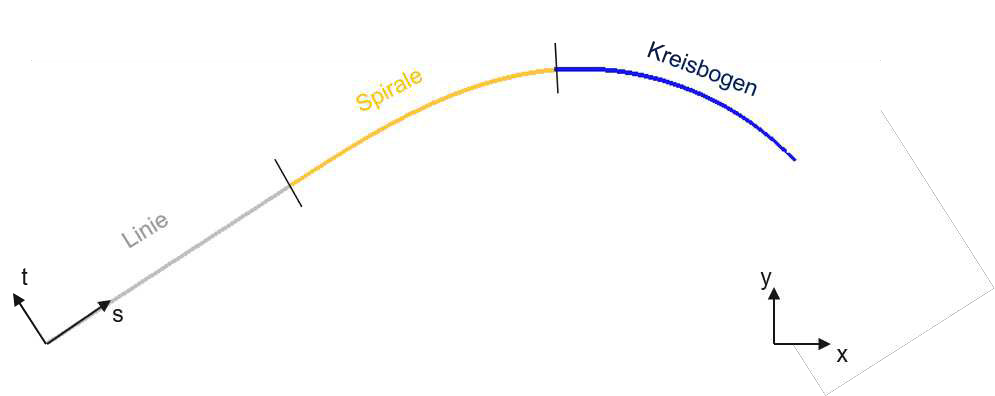
\includegraphics[width=0.95\textwidth]{fig/fig2.png}
\caption{Beispielhafte Referenzlinie im s-t-z Koordinatensystem \cite{Becker.2017}}
\label{abb2}
\end{figure}

An die definierte Referenzlinie können dann während der Streckengenerierung Fahrbahnen hinzugefügt werden, für welche individuelle Breiten oder Markierungen festgelegt werden können. Die Verbindung von mehreren auf diese Weise definierten Strassen ermöglicht letztendlich die Darstellung komplexer Strekennetze und gewährleistet somit eine eindeutige Streckenbeschreibung. 

% --- OPEN DRIVE STANDARD ------------------------------------------------------
\chapter{OpenDRIVE Standard}

OpenDRIVE ist ein 2005 entwickeltes Format zur Darstellung von logischen Straßennetzwerken und gilt mittlerweile als Standard für Streckenbeschreibungen in Fahrzeugsimulationen. Das Format enthält nicht nur Straßen und Fahrbahninformationen, sondern ermöglicht auch die Definition komplexerer Beschilderungen, Fahrbahnmarkierungen oder Ampelsignale. \cite{OpenDRIVE.2019} Definiert wird die OpenDRIVE Datenstruktur im XML-Format in welcher grundsätzlich zwischen Straßen (\texttt{roads}) und Verbindungsstücken (\texttt{junctions}) unterschieden wird. Eine vereinfachte Übersicht der OpenDRIVE Struktur lässt sich in Abbildung \ref{abb3} finden. Hieraus wird deutlich, dass Straßen sowohl direkt, als auch über \texttt{junctions} miteinander verbunden werden können. 

Die Referenzlinie einer jeden Straße wird wie erläutert mit geometrischen Elementen analytisch beschrieben, wobei zusätzlich die laterale Position und Ausrichtung, sowie das Höhenprofil der Straße definiert werden können. Hinzugefügt werden der Straße dann einzelne Fahrbahnen (\texttt{lanes}). Zudem lassen sich unbegrenzt Objekte wie Ampeln oder Schildern definieren. \cite{OpenDRIVEDoku.2019} Das openDRIVE Format ist somit beliebig erweiterbar und ermöglicht dadurch die eindeutige Beschreibung jeder möglichen Strecke. Durch die hohe Komplexität des Formats wird dieses bei großen Streckennetzen für einen Nutzer aber kaum von Hand generierbar.

\begin{figure}[H]
\flushleft
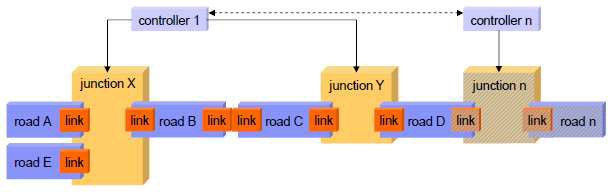
\includegraphics[width=0.95\textwidth]{fig/fig3.png}
\caption{Vereinfachte OpenDRIVE Struktur \cite{Dupuis.2006}}
\label{abb3}
\end{figure}

Deshalb existieren Tools mit denen ermöglicht wird eine Strecke über eine grafische Benutzeroberfläche im OpenDRIVE Format zu erzeugen. Ein Beispiel hierfür ist der \texttt{Road Generator}.\cite{RoadGenerator.2019} Zur Abbildung der Realität kann ein solcher graphischer Generator herangezogen werden, allerdings ist die generische Variierbarkeit von Strecken durch einfache Parameteränderungen ein großer Vorteil bei der Simulation von Fahrmanövern die zur Absicherung durchgeführt werden. 

% --- Abstraktionslevel von Strecken ------------------------------
\chapter{Abstraktionslevel von Strecken}

Im Allgemeinen gibt es verschiedene Möglichkeiten eine Strecke zu beschreiben, wobei sich die hier dargestellten Abstraktionslevel aus der Szenariobeschreibung ableiten lassen. Besonders wichtig ist im Bezug auf diese Arbeit der Unterschied von logischen und konkreten Strecken.

In beiden Beschreibungen wird die Strecke durch Parameter definiert, die die Strecke definieren. Diese Parameter können beispielsweise Kurvenradien oder Spurbreiten sein. Für alle Parameter wird in einer logischen Beschreibung ein Wertebereich festgelegt, sodass sich damit ein Zustandsraum für mögliche, valide Strecken ergibt. Eine konkrete Strecke ist nun eine bestimmte Strecke aus diesem Zustandsraum mit konkreten Parametern, welche durch eine valide logische Beschreibung ebenfalls valide ist.\cite{Szenarienbeschreibung.2019}

Das in diser Arbeit entwickelte Tool soll nun anhand von einer logischen Streckenbeschreibung und zusätzlichen Benutzereingaben eine valide konkrete Strecke erzeugen. Ziel dabei ist, durch kleine Parameteränderungen des Nutzers komplett unterschiedliche konkrete Strecken zu generieren. Dies ermöglicht dann auf einfache Weise die Generierung von beliebig vielen Strecken.

% --- ANNAHMEN UND VEREINFACHUNGEN IM IKA KONZEPT ------------------------------
\chapter {Annahmen und Vereinfachungen im ika Konzept}

Das Tool basiert auf einer logischen Streckenbeschreibung, sodass unabhängig von den gewählten Parametern des Nutzers immer valide Streckennetzte generiert werden. Die konkrete Beschreibung der Strecke hängt dann neben der logischen Beschreibung ebenfalls von den zusätzlich festgelegten Parametern des Nutzers ab. 

Das Tool ermöglicht dabei eine benutzerfreundliche Definition der Streckenparameter, denn nicht alle Werte müssen genau spezifiziert werden. Für viele Abhängigkeiten werden Annahmen getroffen und Standardwerte gesetzt. Trotzdem ist eine Definition von vielen Parametern optional weiterhin über das Eingabedokument möglich. Einige Beispielhafte Annahmen werden im folgenden vorgestellt.

Anders als im OpenDRIVE Format werden Kreuzungen vom Nutzer nur über die Ausgangsstraßen und einem gemeinsamen Kreuzungspunkt definiert, die Definition der Verbindungsstraßen im Kreuzungsbereich sind nicht zwingend notwendig, denn diese werden durch das Tool automatisch erstellt. Dazu wird der Kreuzungsbereich um den Kreuzungsmittelpunkt in einem optional anzugebenen Parameter aufgeschnitten und die verbleibenden Kreuzungsarme durch automatisch berechnete Verbindungsstraßen verbunden.

Weiterhin werden Linksabbiegerspuren auf Hauptstraßen automatisch erstellt und entsprechend Spurmarkierungen gesetzt. Optional können beliebig weitere Eigenschaften der Kreuzung durch den Nutzer spezifiziert werden. So sind zusätzliche Spuraufweitungen für Rechts- oder Linksabbiegerspuren möglich oder Kreuzungssperrbereiche können definiert werden. Eine Spuraufweitung kann dabei mit oder ohne Verschwenkung und nach innen oder außen realisiert werden. Diese beispielhaften erweiterten Kreuzungseigenschaften können im Eingabedokument optional spezifiert werden. Das Tool übersetzt dann aus einer kurzen Angabe einer Spuraufweitung eine komplexe openDRIVE Struktur im Ausgabeformat, in welcher ein neuer Fahrbahnabschnitt mit neuer in breite variierbarer Fahrbahn entsteht. Für den Nutzer händisch wäre eine solche Änderungen nur schwer und sehr aufwendig realisierbar. Mithilfe der vereinfachten Annahmen und den Parametern im Eingabeformat lassen sich so beliebig viele konkrete Strecken generieren.

Zudem muss der Benutzer keine expliziten Koordinaten der Straßen angeben, da die Annahme getroffen wird, dass der Kreuzungsmittelpunkt im Ursprung des kartesischen Koordinatensystems liegt. Darüber hinaus gibt es die Möglichkeit verschiedene Kreuzungssegmente über zwei klar definierte Straßenpunkte miteinander zu verbinden. Über die Koordinaten und die Winkel der Straßen ist die Lage der beiden Segmente dann eindeutig bestimmt. Das Tool transformiert die das entsprechende Segment, sodass das Verbinden von mehreren Elementen und somit die Erstellung komplexer Strassennetze ermöglicht wird.

Um ein Straßennetzwerk schließen zu können bedarf es einer sehr genauen Konstruktion des letzten Segmentes, welches sich in einem überbestimmten Problem widerspiegelt. Deshalb wird zum Schließen eines Netzwerks eine separate Funktion entwickelt, die zwei Punkte unter entsprechendem Winkel miteinander verbindet. Dabei wird angenommen, dass die genaue Geometrie des letzten Segments nicht von großer Bedeutung ist. Die genaue Entwicklung dieser Funktion ist ebenfalls Inhalt der zugrundeliegenden Masterarbeit \cite{Russ.2019}.

Für den Nutzer sind also nur vereinfachte Angaben wie der Kreuzungstyp, die Straßengeometrie, der Kreuzungsschnittwinkel oder die Fahrbahnanzahl gefragt. Das Tool trifft nun Annahmen und Vereinfachungen, sodass basierend auf diesen die Übersetzung in ein detailreiches Straßennetzwerk im gängigen OpenDRIVE Format möglich wird.

% --- UMSETZUNG UND IMPLEMENTIERUNG DES TOOLS ----------------------------------
\chapter{Umsetzung und Implementierung des Tools}
Der folgende Abschnitt beschreibt die grobe Umsetzung des beschriebenen Tools. 

\section{Ein - und Ausgabeformat}
Die Definition des Eingabeformat geschieht ebenfalls wie die Darstellung des OpenDRIVE Formats mithilfe einer XML-Struktur. Dies erlaubt eine übersichtliche Definition der Datenstruktur mit XML Attributen und Elementen. Das Tool zur Generierung des OpenDRIVE Formats wird in \texttt{C++} geschrieben, sodass eine kompatible Bibliothek zum Einlesen und Schreiben der XML-Dateien verwendet wird. Die Bibliothek \texttt{pugi\_xml}\cite{pugixml.2019} ermöglicht das Einlesen der Eingabedatei und speichert die XML-Struktur ähnlich einer Baumstruktur zur Laufzeit, was entsprechend eine effiziente und übersichtliche Verwendung der Eingaben innerhalb des Tools ermöglicht. Ebenso wird eine solche XML-Stuktur zur Laufzeit des Tools erzeugt, die dann mit den generierten OpenDRIVE Objekten gefüllt werden kann.

Ein weiterer Vorteil bei der Benutzung von XML Datenstrukturen ist die Möglichkeit XML Schemata (XSD) zu nutzen. Eine XSD Datei beschreibt die Struktur eines XML Dokumentes, sodass das Auftreten von Attributen und Elementen eingeschränkt werden kann. So besteht beispielsweise die Möglichkeit die Anzahl von Elementen einzuschränken, die Anordnung von Elementen innerhalb des XML Dokuments zu bestimmen oder Attribute nur optional vorzuschreiben. So wurde im Rahmen der Seminararbeit ein XML-Schema Dokument zur Absicherung von falschen Benutzereingaben erstellt. Das verwendete OpenDRIVE Format besitzt ebenfalls eine solche Schemadatei, sodass sowohl Eingabe als auch Ausgabedokument des Streckengenerators mithilfe eines \texttt{XML/XSD}Validierungstools abgesichert werden können. Im Zuge der Arbeit wurde hierfür die Bibliothek \texttt{xerces-c}\cite{Xerces.2019} verwendet.

\section{Implementierung}
Die Implementierung des in \texttt{C++} entwickelten Tools gliedert sich ebenfalls in die drei schematisch beschriebenen Entwicklungsschritte. Im ersten Schritt werden die Segmente (Kreuzungen, Kreisverkehre oder Verbindungsstraßen) basierend auf den Angaben in der Eingabedatei generiert. Im Anschluss werden diese Segmente dann wie vom Benutzer definiert miteinander verbunden bevor im letzten Schritt Straßen zum Schließen des Streckennetzwerkes generiert werden.

\subsection{Generierung der Segmente}

Die Eingabedaten werden zur Laufzeit eingelesen und sind so global innerhalb des Tools verfügbar. Im Folgenden wird beispielhaft der Entwicklungsprozess einer X-Kreuzung genauer beschrieben.

Für eine X-Kreuzung existieren drei verschiedene Fälle wie in Abbildung \ref{abb4} dargestellt, welche sich in Anzahl und Anordnung der definierten Eingangsstraßen unterscheiden.

\begin{figure}[H]
\flushleft
\includegraphics[width=0.95\textwidth]{fig/fig4.tikz}
\caption{Unterschiedliche Arten einer X-Kreuzung}
\label{abb4}
\end{figure}

Abhängig vom definierten Kreuzungstyp werden die entsprechend relevanten Straßen und die zugehörigen Informationen wie beispielsweise die definierten Kreuzungsbereichgröße aus dem XML Dokument eingelesen. Im nächsten Schritt werden vier Ausgangsstraßen der X-Kreuzung basierend auf den Eingangsstraßen generiert, welche sich entsprechend dem definierten Winkel anordnen lassen. Die generische Funktion \texttt{generateRoad} erstellt dabei eine Straße ausgehend vom bestimmtem Hauptpunkt im Kreuzungsbereich. Die positive s Koordinatenrichtung zeigt dabei immer weg vom Kreuzungsmittelpunkt. Zudem werden für Hauptstrassen automatisch Linksabbiegerspuren oder Ampelanlagen eingefügt. Falls der Nutzer weitere Angaben macht, wie beispielsweise zusätzliche Spuraufweitungen, werden diese ebenfalls umgesetzt und im openDRIVE Format generiert.

Nach erfolgreicher Erstellung der vier Ausgangsstraßen werden die Straßen im Kreuzungsbereich erstellt. Der Benutzer hat die Möglichkeit alle Fahrbahnen automatisch und logisch miteinander zu verbinden oder selbst Verbindungsstraßen zu spezifizieren. Beim Definieren einer Fahrbahn ist darauf zu achten, dass sich mögliche Unterschiede im lateralen Abstand oder der Spurbreite kontinuierlich ausgleichen. Dabei wird die Breite einer Spur im openDrive Format stets über eine kubische Funktion über die longitudinale s Richtung definiert. Dabei ist stets auf einen stetigen Übergang ohne Krümmungsprung zu achten. Die Funktion \texttt{createRoadConnection} verbindet die Fahrbahnen mit einer Verbindungsstraße. Das Polynom für die Breite oder laterale Offsets werden dabei automatisch berechnet. Im Anschluss werden zusätzlich vorgegebene Fahrbahnmarkierungen hinzugefügt.

Im Kreuzungsbereich besitzt jede angelegte Straße als Vor- und Nachfolger eine \texttt{junction}, welche ebenfalls innerhalb der Funktionen festgelegt und definiert werden. Die zugrundeliegende Struktur lässt sich nochmals in Abbildung \ref{abb3} erkennen. Die Verbindungen zwischen den Straßen ermöglichen eine valide Struktur, sodass jede Straße über die Verbindung auch ihre Vor- und Nachfolger kennt.

Analog werden auch die weiteren Segmente wie beispielsweise eine T-Kreuzung, ein Kreisverkehr oder auch eine einfache Umgehungsstraße generiert und in einer global verfügbaren Datenstruktur im OpenDRIVE Format abgespeichert.

\subsection{Anordnung der Segmente}

Durch den Benutzer wird in der Eingabedatei das Referenzsegment mit Position und Ausrichtung festgelegt. Alle Geometrien dieses Segments werden also innerhalb des Tools um den definierten Winkel gedreht und entlang der x-y Achsen verschoben, sodass sich der Ursprung des Segments (Kreuzungsmittelpunkt) an der definierten Position befindet.

Weiterhin gibt der Nutzer Straßenpunkte zweier unterschiedlicher Segmente an, die miteinander verbunden werden sollen. Innerhalb der Funktion \texttt{linkSegments} wird dann der Winkel um den gedreht werden muss und die x-y Werte der Verschiebung bestimmt, sodass nach Transformation der Geometrien des neuen Segments die Endpunkte der zwei Segmente ohne Winkelsprung aufeinander liegen.

\subsection{Verbinden der Segmente}

Im letzten Schritt werden automatisch Straßen generiert, die zwei beliebige Endpunkte zweier Segmente miteinander verbinden, was im Entwicklungsprozess zum Schließen eines Streckennetzwerkes erforderlich ist. Die verantwortliche Funktion \texttt{closeRoadConnection} berechnet hierbei aus den Koordinaten und Richtungen der Straßenendpunkte die Verbindungsstrecke. Dazu wird der Schnittpunkt der beiden Richtungsvektoren gebildet und unterschieden, ob der Schnittpunkt auf positiver oder negativer Seite des Schnittpunktes liegt. Dies führt letztendlich zu neun verschiedenen Fällen, je nach Ausrichtung der beiden zu verbindenden Punkte. Falls eine direkte Verbindung mithilfe einer Geraden und einer Verbundkurve nicht möglich ist, wird ein Hilfspunkt eingefügt, die Strecke bis dahin mit Gerade oder Kreisbogen erweitert und entsprechend mit den neuen Punkten die Funktion \texttt{closeRoadConnection} rekursiv aufgerufen. Der Fall, dass die Punkte direkt miteinander verbunden werden können, lässt sich in zwei Unterfälle teilen.

Zum einen ist dies möglich, falls beide Vektoren in die gleiche Richtung und der Startvektor auf den Endvektor zeigt. Für diesen trivialen Fall lässt sich das Stück mit einer einfachen Geraden verbinden.

Für den Fall, dass der Schnittpunkt in positiver Richtung des Startvektors und in negativer Richtung des Endvektors liegt lässt sich die Strecke ebenfalls verbinden. Dazu wird der Abstand von Start und Endpunkt zum Schnittpunkt verglichen und das längere Stück so weit mit einer Geraden verlängert, bis Start und Endpunkt gleich weit vom Schnittpunkt entfernt liegen. Nun lässt sich das fehlende Stück mithilfe eines Kreisbogens schließen. Für kleine Geschwindigkeiten wird hierbei der Krümmungssprung zwischen Gerade und Kreisbogen toleriert. Die Berechnung des Kreisbogens erfolgt mit der Konstruktion eines Gleichschenkligen Dreiecks wie in Abbildung \ref{abb5} dargestellt. Hierbei beschreiben die beiden roten Punkte mit Vektoren \(A\) und \(B\) die Ausgangspunkte, der blaue Punkt den Schnittpunkt und der orange Punkt den hinzugefügten Hilfspunkt.

\begin{figure}[H]
\flushleft
\begin{subfigure}{0.32\textwidth}
    \vspace{1.2cm}
    \includegraphics[width=0.95\textwidth]{fig/fig5a.tikz}
    \caption{Konstruktion des Hilfspunktes}
\end{subfigure}
\begin{subfigure}{0.32\textwidth}
    \includegraphics[width=0.95\textwidth]{fig/fig5b.tikz}
    \caption{Konstruktion des Kreissegments}
\end{subfigure}
\begin{subfigure}{0.32\textwidth}
    \vspace{1.65cm}
    \includegraphics[width=0.95\textwidth]{fig/fig5c.tikz}
    \caption{Konstruierte Verbindung der beiden Punkte \(A\) und \(B\)}
\end{subfigure}
\caption{Vorgehen beim Verbinden zweier Straßenendpunkte}
\label{abb5}
\end{figure}

Der Radius des Kreises lässt sich nun über folgende Beziehung herleiten.
\begin{align}
\text{sin}(\frac{\alpha}{2}) &= \frac{\frac{d}{2}}{R} \\
&\Rightarrow \hspace{2cm} R = \frac{d}{2 \cdot \text{sin}(\frac{\alpha}{2})} \\
&\Rightarrow \hspace{2cm} l = R \cdot \alpha
\end{align}

Mit berechnetem Kreisradius und dem zu überbrückenden Winkel \(\alpha\), kann  ebenfalls die Länge des Kreissegments bestimmt werden. Somit ist der Kreis, welcher die fehlende Lücke schließt klar definiert und das Straßensegment geschlossen.

Für den Fall, dass die Straße an Start oder Endpunkt eine Krümmung besitzt, wird automatisch ein Spiralsegment eingefügt, welches den Krümmungssprung überbrückt. Ein weiterer Ausgleich ist erforderlich, falls die Anzahl der Spuren oder die Spurbreite zwischen Start und Endpunkt variiert. Dieses Verfahren findet ebenfalls beim automatischen Verbinden zweier Straßen im Kreuzungsbereich Anwendung.

Das Vorgehen gewährleistet einen kontinuierlichen Übergang vom Startpunkt in den Endpunkt und somit ein korrektes Schließen des Straßennetzwerkes. Zusammen mit den anderen gezeigten Funktionen bildet das Tool also eine Möglichkeit beliebige Straßennetze zu konstruieren und im OpenDRIVE Format abzuspeichern. Diese sind dann nutzbar für weitere Simulationen.

% --- BEISPIELE UND TESTS ------------------------------------------------------
\chapter{Beispiele und Tests}

Im folgenden Abschnitt finden sich einige beispielhaft generierte Kreuzungen. Zudem wurden im letzten Schritt einige zuvor generierte Straßen zusammengefügt und durch Verbindungsstraßen mithilfe der Funktion \texttt{closeRoadConnection} geschlossen.

\section{X-Kreuzung}
Wie schon erläutert gibt es für Kreuzungen verschiedene Typen. Der hier beispielhaft gezeigte Typ besteht aus einer durchgehenden Hauptstraße und zwei aneinandergrenzenden Nebenstraßen. Verbunden werden sollen alle Fahrstreifen im Kreuzungsbereich und die Kreuzungsbereichgröße wird auf \(15 m\) in alle Richtungen gesetzt. Per Definition befindet sich der Kreuzungsmittelpunkt im Ursprung des kartesischen Koordinatensystems. Eine Darstellung der beispielhaften Kreuzung befindet sich in Abbildung \ref{abb6}.

\begin{figure}[H]
\flushleft
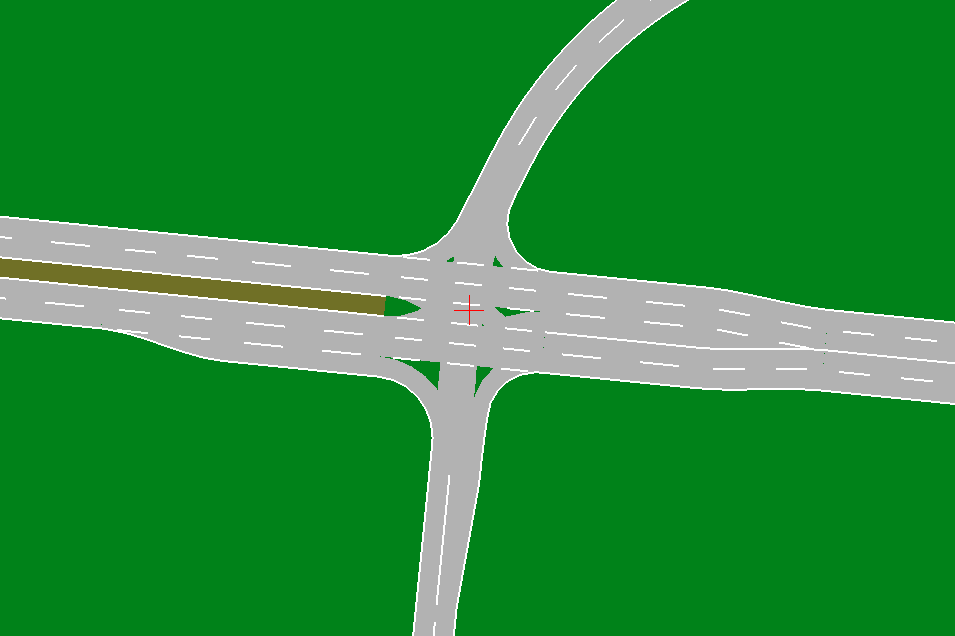
\includegraphics[width=0.95\textwidth]{fig/junction4.png}
\caption{X-Kreuzung im OpenDRIVE Viewer}
\label{abb6}
\end{figure}

Zusätzlich wurden im Eingabedokument weitere Abbiegespuren und Sperrbereiche definiert. Auf der Hauptstraße wurde eine Linksabbiegerspur mit Verschwenkung und gegenüber ein entsprechender Sperrbereich definiert. Des weiteren existieren zwei unterschiedliche Typen von Rechtsabbiegerspuren. Auf der Hauptstraße ist eine einmalige Aufweitung zu Beginn vorzufinden, wärend auf der Nebenstraße eine linear aufweitende Spuraufweitung definiert wurde. 

Automatisiert werden alle relevanten Spuren miteinander verbunden. Das Beispiel zeigt also eine konkrete und valide Kreuzung generiert aus einfachen Eingabedaten, denn der Nutzer gibt neben den Gemometrien der drei Eingangsstraßen nur den Schnittwinkel und die Abbiegespuren an. Dies macht sich auch bemerkbar wenn die Ein- und Ausgabedokumente näher untersucht werden. 

Das vereinfachte Eingabeformat enthält für diesen konkreten Fall \(55\) Zeilen die für den Nutzer leicht zu verstehen und übersichtlich sind, während das openDrive Ausgabedokument \(1091\) Zeilen enthält, in welchem die Straßen und Verbindungselemente hintereinander gelistet sind. Der Vorteil des Tools wird daraus klar ersichtlich, weil es eine intuitive Definition von Kreuzungen im openDrive Format ermöglicht. 

\section{T-Kreuzung}
Analog zur X-Kreuzung kann auch eine T-Kreuzung generiert werden. Der hier dargestellte Typ besteht hierbei aus einer Hauptstrasse und einer angrenzenden Nebenstraße. Auf der Hauptstraße wurde automatisch eine Linksabbiegerspur und entsprechend ein gegenüberliegender Sperrbereich generiert. Eine Übersicht der erläuterten Kreuzung lässt sich in Abbildung \ref{abb7} finden.

\begin{figure}[H]
    \flushleft
    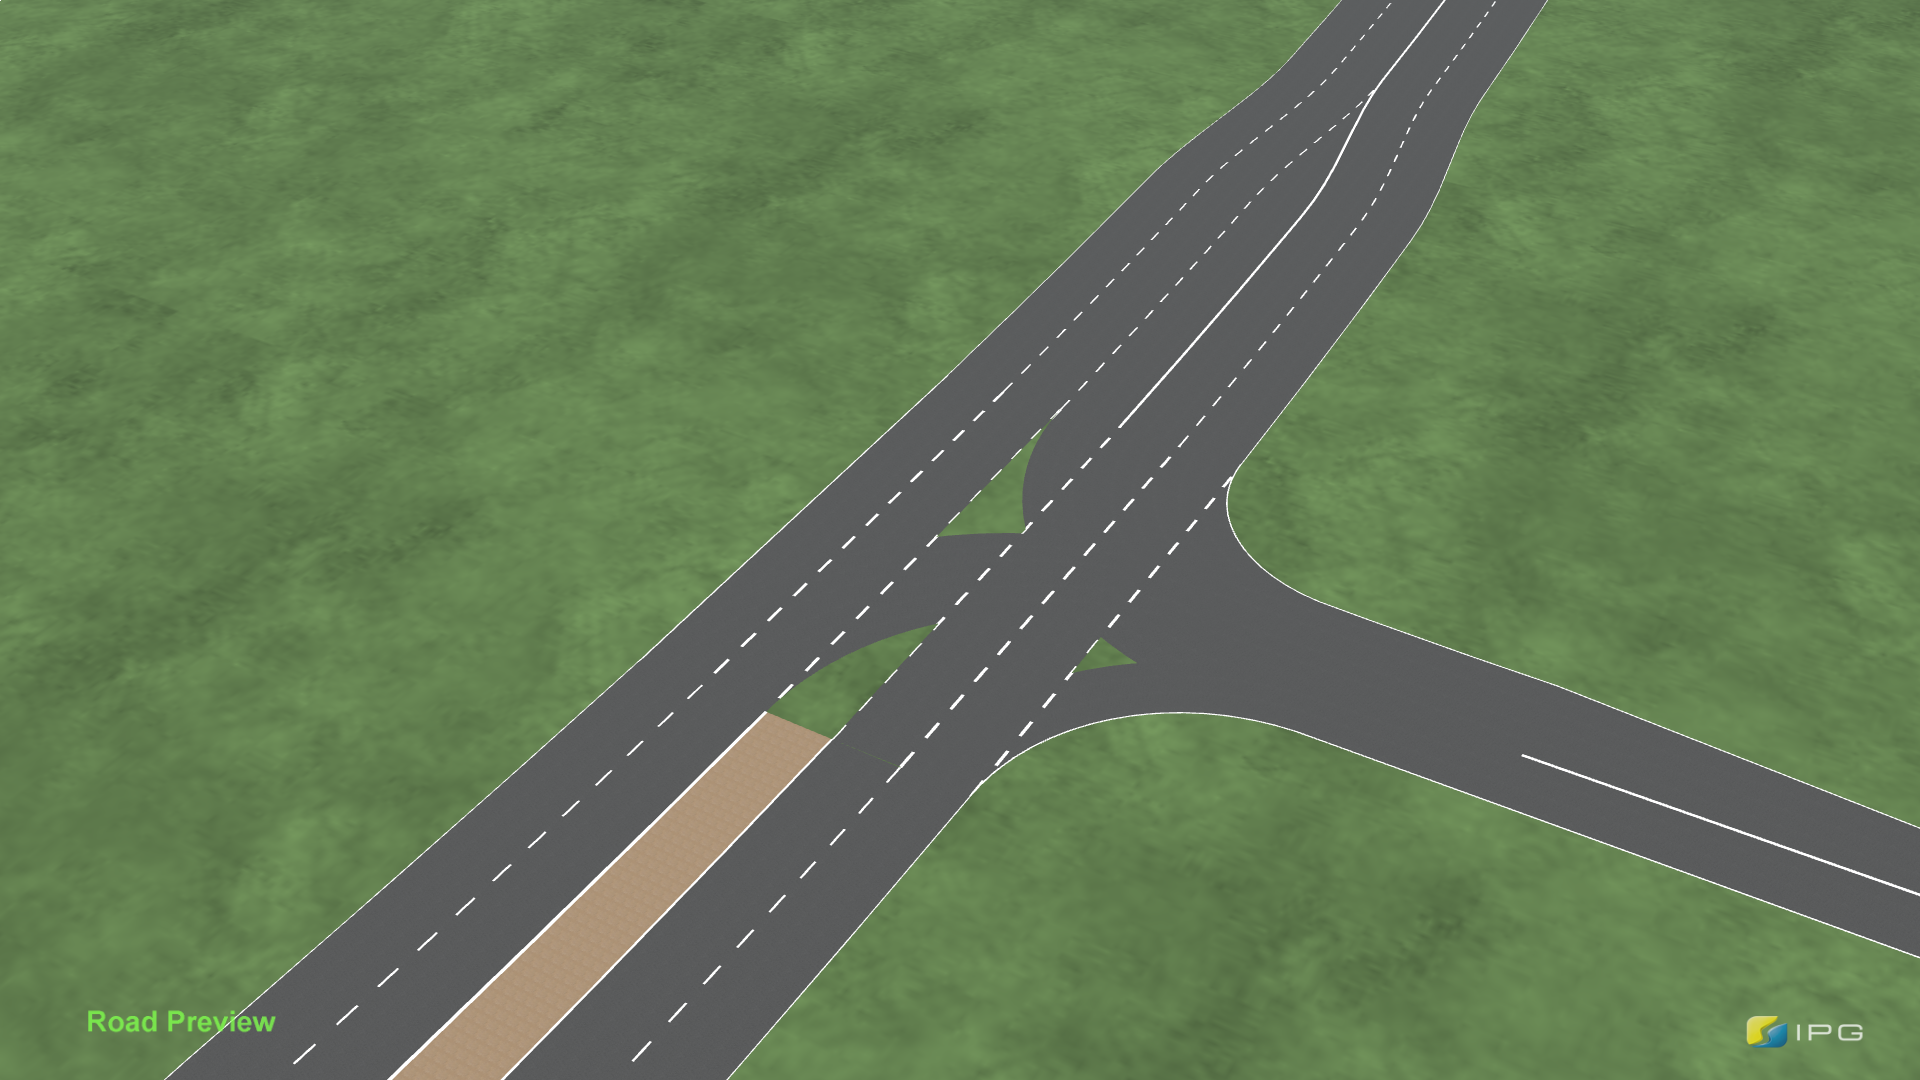
\includegraphics[width=0.95\textwidth]{fig/junction6.png}
    \caption{X-Kreuzung im OpenDRIVE Viewer}
    \label{abb7}
\end{figure}

Auch hier wird aus einfachen Eingabedaten mit lediglich \(44\) Zeilen eine komplexe openDRIVE Struktur mit \(461\) Zeilen generiert. Zusätzlich ist für den Nutzer das Eingabeformat des Tools intuitiver und übersichtlicher.

\section{Kreisverkehr}
Neben Kreuzungen können auch Kreisverkehrsegmente erstellt werden, welche an sich, als Zusammenschluss von einzelnden T-Kreuzungen verstanden werden können. Ausgangspunkt ist die Definition des Kreises mit Radius und Spuranzahl, sowie der angrenzenden Straßen mit jeweiliger Position und Winkel der Schnittpunktes. Daraus generiert das Tool alle Kreuzungsbereiche des Kreisverkehrs eigenständig, schneidet das Kreissegment an den entsprechenden Stellen und erstellt die Verbindungsstraßen der einzelnen T-Kreuzungen. Eine Visualisierung der Straßen lässt sich in Abbildung \ref{abb8} finden. Zudem werden automatisch Verkehrsschilder und Fahrbahnmarkierungen erstellt.

\begin{figure}[H]
\flushleft
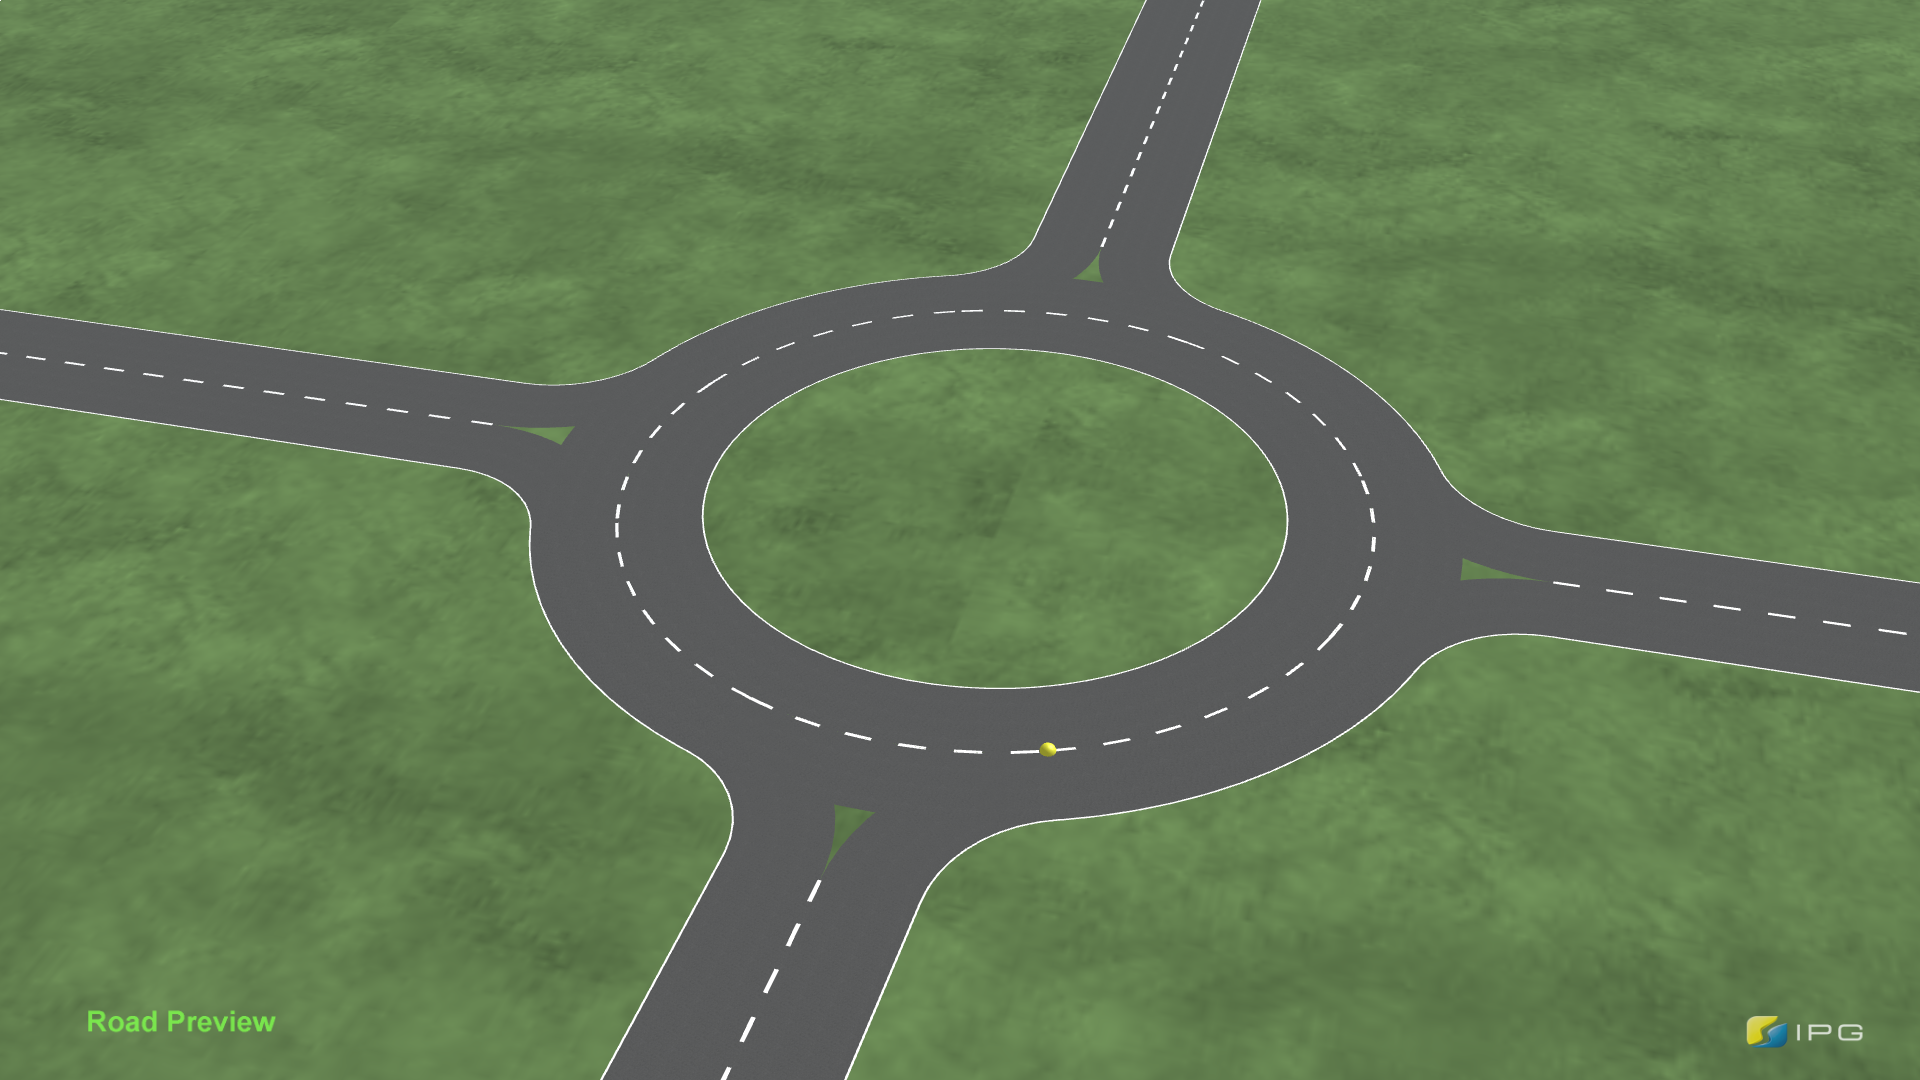
\includegraphics[width=0.95\textwidth]{fig/roundabout.png}
\caption{Kreisverkehr im OpenDRIVE Viewer}
\label{abb8}
\end{figure}

Angrenzend an eine ringförmige Straße treten vier Nebenstraßen auf, die zusammen mit Verbindungsstraßen einen geschlossenen, in sich validen Kreisverkehr ergeben. Hierbei wird das Zeilenverhältnis von \(38\) zu \(988\) zwischen Eingabe- und Ausgabedatei besonders deutlich.

\section{Komplexes Straßennetzwerk}

Diese und weitere parametrisierte Segmente lassen sich mithilfe des erstellten Tools generieren. Das zugrundeliegende Beispiel zeigt nun, dass die Segmente aneinander gefügt werden können und ferner zwei Straßenenden mit einer neu generierten Straße automatisiert miteinander Verbunden werden können. Zwar ist die erstellte Verbindungsstraße nicht immer die kürzeste Möglichkeit zur Verbindung der Straßen, jedoch wird der genaue Verlauf der Verbindungsstraße hierbei vernachlässigt.

\begin{figure}[H]
\flushleft
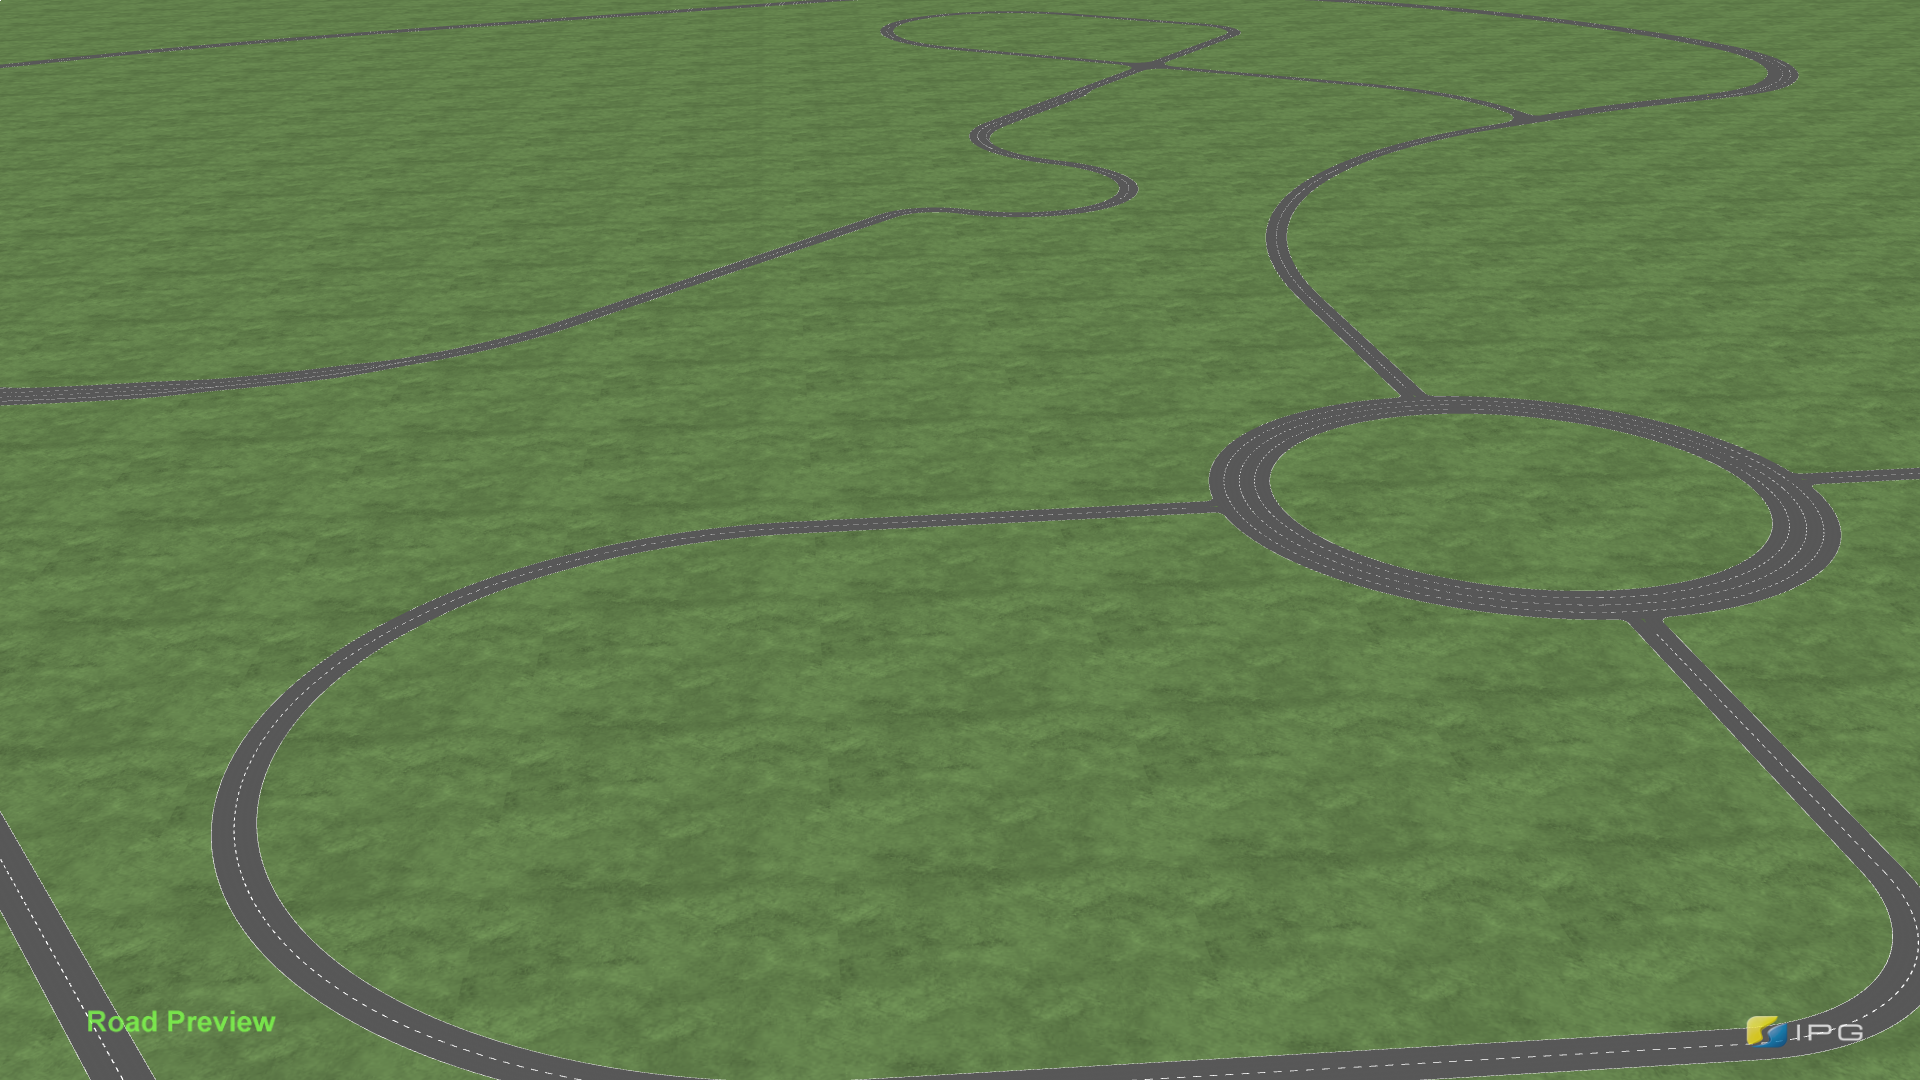
\includegraphics[width=0.95\textwidth]{fig/all.png}
\caption{Streckennetzwerk im OpenDRIVE Viewer}
\label{abb9}
\end{figure}

Die Segmente wurden teilweise über zwei Straßenarme aneinander gefügt, teilweise aber auch automatisch über eine neu angelegte Verbindungsstraße miteinander verbunden. Zudem zeigt das Beispiel, welches in Abbildung \ref{abb9} zu finden ist weitere Funktionen des Tools, wie beispielsweise Spuraufweitungen und Spurverringerungen oder einen Ausgleich von unterschiedlichen Spurbreiten. Zusätzlich sind weitere Elemente einer Strecke wie Verkehrsinseln oder Bushaltestellen zu finden. Das Verhältnis der Zeilen kann hier ebenso untersucht werden und ist mit \(248\) zu \(5191\) ebenfalls sehr deutlich.

\section{Auswertung}

Die Beispiele haben gezeigt, dass durch die getroffene logische Beschreibung und kurzen, aussagekräftigen Parametern eine konkrete Streckenbeschreibung im openDRIVE Format möglich wird. Das Verhältnis von Eingabe und Ausgabeformat wird in Tabelle \ref{tab1} noch einmal veranschaulicht.
\begin{figure}
    \centering
    \begin{tabular}{c|c|c|c}
        \toprule
        \textbf{Beispielfall} & Zeilen in Eingabedatei & Zeilen in Ausgabedatei & Faktor \\
        \midrule
        T-Kreuzung   & 44 & 461  & 10.47\\
        X-Kreuzung   & 55 & 1091 & 19.84\\
        Kreisverkehr & 38 & 988 & 26.00\\
        Straßennetz  & 248 & 5191 & 20.93 \\
        \bottomrule
    \end{tabular}            
    \caption{Verhältnis der Zeilenanzahl von Eingabe und Ausgabedokument}
    \label{tab1}
\end{figure}

Der Faktor zwischen Eingabe und Ausgabedatei liegt hier im Durchschnitt bei \(19.31\).

Interessant ist auch der Einfluss einer kleinen Parameteränderung. Wird beispielsweise der Winkel des Referenzsegments nur im Vorzeichen geändert ergibt dies für den letzten Beispielfall direkt eine Änderungen von \(188\) Zeilen in der openDrive Datei.

Der Aufwand für eine solche Änderung wäre manuell also kaum umsetzbar, das Tool hingegen kann auf diese Weise beliebig viele konkrete Streckenbeschreibungen generieren.

Insgesamt zeigen die dargestellten Beispiele, dass das Tool die vereinfachten Eingaben des Nutzers, zusammen mit der logischen Beschreibung in ein valides und generisches Straßennetz im OpenDRIVE Standard übersetzen kann.

% --- AUSBLICK -----------------------------------------------------------------
\chapter{Ausblick}

Das in dieser Seminararbeit entwickelte Tool ermöglicht es mithilfe einer logischen Streckenbeschreibung ein vollständiges und konkretes Streckennetz im standardisierten OpenDRIVE Format zu generieren. Dies erlaubt Benutzern durch einfache Parameteränderungen komplett unterschiedliche, aber valide, konkrete Strecken zu erhalten. So ist es möglich große Strecken mit wenigen Eingaben zu generieren und für eine anschließende Simulation zu benutzen.

Im Rahmen der Arbeit wurde der Streckengenerator in \texttt{C++} entwickelt und für die aufgezählten Kreuzungssegmente implementiert. Grundsätzlich lag der Fokus dabei auf innerstädtische Streckenbereiche und somit auf Kreuzungen, was durch weitere Annahmen aber ebenfalls auf Autobahnen ausgeweitet werden könnte. Zudem können auch innerstädtisch weitere Funktionen eingebaut werden, die dann weitere Szenarien abdecken. Beispiele hierfür sind Fußgängerüberwege oder Bürgersteige. Letztendlich ist durch das offen gehaltene OpenDRIVE Format jedes mögliche Szenario auch mithilfe des Generators in eine valide konkrete Strecke umsetzbar.
